\documentclass[10pt,a4paper]{report}
\usepackage[utf8]{inputenc}
\usepackage[english]{babel}
\usepackage{amsmath}
\usepackage{amsfonts}
\usepackage{amssymb}
\usepackage{listings}
\usepackage{xcolor}   % required for colour definitions

% Define colours (feel free to adjust)
\definecolor{codegreen}{rgb}{0,0.6,0}
\definecolor{codegray}{rgb}{0.5,0.5,0.5}
\definecolor{codepurple}{rgb}{0.58,0,0.82}
\definecolor{backcolour}{rgb}{0.95,0.95,0.92}
\definecolor{codered}{rgb}{0.8,0.04,0.18}
\definecolor{codeblue}{rgb}{0.12,0.29,0.53}

% Global settings for all listings
\lstset{
    language=C,                 % default language
    basicstyle=\ttfamily\small, % font style and size
    backgroundcolor=\color{backcolour}, % light background
    commentstyle=\color{codegreen},     % green comments
    keywordstyle=\color{codeblue}\bfseries, % blue keywords
    stringstyle=\color{codered},        % red strings
    identifierstyle=\color{black},
    numberstyle=\tiny\color{codegray},
    stepnumber=1,
    numbersep=5pt,
    tabsize=4,
    showspaces=false,
    showstringspaces=false,
    frame=single,               % adds a frame around the code
    captionpos=b,               % caption at the bottom
    breaklines=true,            % automatic line breaking
    breakatwhitespace=false,
    escapeinside={\%*}{*)},     % if you need to add LaTeX inside
    numbers=left,               % line numbers on the left
    xleftmargin=2em,
    framexleftmargin=1.5em,
}
\usepackage{graphicx}
\usepackage{comment}
\usepackage[left=2cm,right=2cm,top=2cm,bottom=2cm]{geometry}
\author{Burduja Adrian}
\title{Lab1}

\begin{document}

\maketitle

\section*{Laboratory 1.1}

\subsection*{Domain analysis}

For this laboratory I used various software and hardware technologies.
For software, I used various websites in order to learn how to implement the
necessary functionalities: youtube,claude,deepseek.
For implementing the project itself, I used simulators for testing:SimulIDE,
and a suite for compiling the code: Arduino-cli.
For help with some aspects, I prompted various LLM's with questions on how
to implement certain functionalities, like how to link the stdin/stdout to the
serial interface, how to control the input/output of the various pins etc. 
Additionally, I also asked for some help on formatting the report itself and 
the last paragraph of the conclusion.

For hardware, I chose Arduino mega, as well as various necessary components. 

\subsection*{Design}
\begin{figure}[!ht]
    
\includegraphics[width=0.8\textwidth]{img/diagram.png}
    \caption{Architectural sketch}
\end{figure}
\begin{figure}[!ht]
    \begin{minipage}{0.45\textwidth}
        \centering
        
\includegraphics[width=\textwidth]{img/block.png}
        \caption{Block diagram}
    \end{minipage}
    \hfill
    \begin{minipage}{0.45\textwidth}
        \centering
        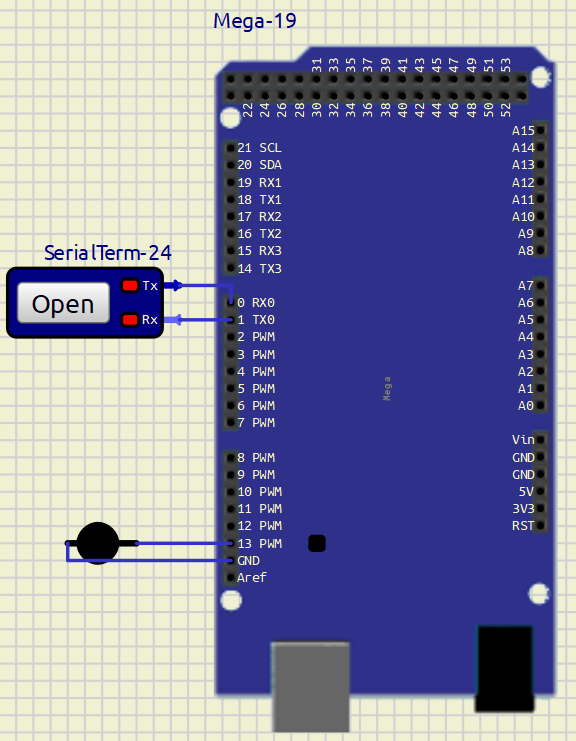
\includegraphics[width=\textwidth]{img/circuit.png}
        \caption{Circuit diagram}
    \end{minipage}
\end{figure}

\subsubsection*{Sample input/output example of usage}
\begin{lstlisting}
// terminal input
gibberish
led on
led off

// terminal output
Unknown command:gibberish

Led on
Led off
\end{lstlisting}

\subsection*{Conclusion}
The implemented system executes the necessary functions: turning on/off a LED based on user input to a terminal, as well as using
STDIO to communicate with the terminal. The implementation is specific for 
the particular hardware, components and their connections. The modular 
architecture clearly separates main functionality, string processing and 
handling STDIO setup.

In conclusion, the implemented system works as expected: it correctly parses
user input and turns on or off the LED based on the imputed command, else it
just reports back to the user the incorrect or non-existent command.

Beyond the laboratory, the technologies used have direct real-world relevance — simulators like SimulIDE accelerate prototyping, Arduino-cli enables automated build pipelines, and LLM-assisted development reflects modern AI-driven workflows. The fundamental technique of remapping standard I/O to a serial interface is a transferable skill found in countless embedded systems, from bootloaders to industrial diagnostics. Thus, the project demonstrates both functional correctness and the practical value of industry-aligned development practices.

\newpage
\begin{thebibliography}{9} % 9 is the widest label expected

\bibitem{arduino}
Arduino,
\emph{Arduino CLI documentation},
https://arduino.github.io/arduino-cli/,
accessed: 2025-02-1.

\bibitem{simulide}
SimulIDE,
\emph{SimulIDE – Real Time Electronic Circuit Simulator},
https://simulide.com/,
accessed: 2025-02-13.

\bibitem{uart}
Wikipedia,
\emph{Universal asynchronous receiver-transmitter},
https://en.wikipedia.org/wiki/Universal\_asynchronous\_receiver-transmitter,
accessed: 2025-02-6.

\bibitem{deepseek}
Deepseek, 
https://chat.deepseek.com
accessed: 2025-02-13

\bibitem{claude}
Claude
https://claude.ai
accessed: 2025-02-6

\end{thebibliography}

\newpage
\section*{Appendix}

\subsection*{main.c}
\begin{lstlisting}
#include <stdio.h>
#include <Arduino.h>
#include "lab11_driver.h"
#include "stdio_layer.h"
#include "strings.h"

int main(void){
	init();
	
	init_led();
	init_stdout();

	init_leds();
	init_keypad();
	
	// loop
	for(;;){

		// lab11 code
		read_input();

		if (turn_on_command()) {
			printf("Led on\n");
			led_turn_on();
		} else if(turn_off_command()){
			printf("Led off\n");
			led_turn_off();
		} else {
			printf("Unknown command:");
			print_input();
			printf("\n");
		}
	}
	printf("End of loop");
	return 0;
}
\end{lstlisting}

\newpage
\subsection*{$lab11\_driver.h$}
\begin{lstlisting}
#pragma once
#include <stdbool.h>

void init_led();
void init_stdout();
void led_turn_on();
void led_turn_off();
bool turn_on_command();
bool turn_off_command();
\end{lstlisting}

\subsection*{$lab11\_driver.c$}
\begin{lstlisting}
#include <avr/io.h>
#include <stdbool.h>
#include <string.h>
#include "stdio_layer.h"

// Register controll
#define LED_REGISTER PB7

void init_led(){
	// set LED_REGISTER'th bit to 1 in data direction register b (DDRB)
	// sets the pin to output mode
	DDRB |= (1 << LED_REGISTER);
}
void led_turn_on(){
	// set LED_REGISTER'th bit to 1 in b port register (PORTB), 
	// sends voltage through the corresponding pin
	PORTB |= (1 << LED_REGISTER);
}
void led_turn_off(){
	// set LED_REGISTER'th bit to 0 in b port register (PORTB), 
	// stops voltage through the corresponding pin
	PORTB &= ~(1 << LED_REGISTER);
}

// Commands
#define ledon_size 6
const char *led_on = "led on";

bool turn_on_command(){
	// returns true if the string in bufflen() is the same as led_on
	return ((bufflen() == ledon_size+1) && (strncmp(buffer(),led_on,ledon_size)==0));
}

#define ledoff_size 7
const char *led_off = "led off";

bool turn_off_command(){
	// returns true if the string in bufflen() is the same as led_off
	return ((bufflen() == ledoff_size+1) && (strncmp(buffer(),led_off,ledoff_size)==0));
}
\end{lstlisting}


\subsection*{$stdio\_layer.c$}
\begin{lstlisting}
#include "stdio_layer.h"
#include <stdio.h>
#include <Arduino.h>
// Code generated by claude
// start

int uart_putchar(char c, FILE *stream) {
	if (c == '\n') { uart_putchar('\r', stream); }
	while(!(UCSR0A & (1 << UDRE0)));
	UDR0 = c;
	return 0;
}

int uart_getchar(FILE *stream) {
	while(!(UCSR0A & (1 << RXC0)));
	return UDR0;
}

FILE uart_str = FDEV_SETUP_STREAM(uart_putchar, uart_getchar, _FDEV_SETUP_RW);

void uart_init(unsigned long baud){
	unsigned int ubrr = F_CPU/16/baud - 1;
	UBRR0H = (ubrr >> 8);
	UBRR0L = ubrr;
	UCSR0B = (1 << TXEN0) | (1 << RXEN0);
	UCSR0C = (3 << UCSZ00);

	stdout = &uart_str;
	stdin = &uart_str;
}

// end

void init_stdout(){ uart_init(9600); }

// IO
#define BUFFER_SIZE 255
char _buffer[BUFFER_SIZE+1];
char* buffer(){return _buffer;}

int _bufflen = 0;
int bufflen(){return _bufflen;}

void read_input(){
	fgets(_buffer, BUFFER_SIZE, stdin);
	_bufflen = strlen(_buffer);
}

void print_input(){ printf("%s", _buffer); }
\end{lstlisting}

\subsection*{$strings.h$}
\begin{lstlisting}
#pragma once
bool string_cmp(const char* lhs, const char* rhs);
\end{lstlisting}

\subsection*{$strings.c$}
\begin{lstlisting}
#include <stdbool.h>
#include <string.h>

bool string_cmp(const char* lhs, const char* rhs){
	return ((strlen(lhs) == strlen(rhs)) && (strncmp(lhs,rhs,strlen(rhs))==0));
}
\end{lstlisting}


%==========%
% template %
%==========%
\begin{comment}
\subsubsection*{}
\begin{lstlisting}
\end{lstlisting}
\begin{figure}[!ht]
    \includegraphics[width=1\textwidth]{q.jpg}
\end{figure}
\end{comment}

\end{document}
